\subsubsection{Abstract}

Automatic differentiation frameworks are optimized for exactly one thing:
computing the average mini-batch gradient. Yet, other quantities such as the
variance of the mini-batch gradients or many approximations to the Hessian can,
\emph{in theory}, be computed efficiently, and at the same time as the gradient.
While these quantities are of great interest to researchers and practitioners,
current deep-learning software does not support their automatic calculation.
Manually implementing them is burdensome, inefficient if done na\"ively, and the
resulting code is rarely shared. This hampers progress in deep learning, and
unnecessarily narrows research to focus on gradient descent and its variants; it
also complicates replication studies and comparisons between newly developed
methods that require those quantities, to the point of impossibility. To address
this problem, we introduce \BackPACK, an efficient framework built on top of
\PyTorch, that extends the backpropagation algorithm to extract additional
information from first- and second-order derivatives. Its capabilities are
illustrated by benchmark reports for computing additional quantities on deep
neural networks, and an example application by testing several recent curvature
approximations for optimization.

\marginnote{%
  \begin{center}
    Code and experiments available at the Github repositories
    \href{https://github.com/f-dangel/backpack}{\texttt{f-dangel/backpack}},
    \href{https://github.com/f-dangel/backpack-experiments}{\texttt{f-dangel/backpack-experiments}}
  \end{center}
  \begin{center}
    
\includegraphics[height = 0.8\linewidth]{../repos/backpack-paper/tex/logo/backpack_logo_github.pdf}
  \end{center}
}%

\section{Introduction}
The success of deep learning and the applications it fuels can be traced to the
popularization of automatic differentiation frameworks. Packages like
\TensorFlow~\citep{abadi2016tensorflow}, \Chainer~\citep{tokui2015chainer},
\MXNet~\citep{chen2015mxnet}, and \PyTorch~\citep{paszke2019pytorch} provide
efficient implementations of parallel, GPU-based gradient computations to a wide
range of users, with elegant syntactic sugar.

However, this specialization also has its shortcomings: it assumes the user only
wants to compute gradients or, more precisely, the average of gradients across a
mini-batch of examples. Other quantities can also be computed with AD at a
comparable cost or minimal overhead to the gradient backpropagation pass; for
example, approximate second-order information or the variance of gradients
within the batch. These quantities are valuable to understand the geometry of
deep neural networks, for the identification of free parameters, and to push the
development of more efficient optimization algorithms. But researchers who want
to investigate their use face a chicken-and-egg problem: AD tools required to go
beyond standard gradient methods are not available, but there is no incentive
for their implementation in existing deep-learning software as long as no large
portion of the users need it.

Second-order methods for deep learning have been continuously investigated for
decades \citep[\eg][]{becker1988improving,amari1998natural,bordes2009sgdqn,
  martens2015optimizing}. But still, the standard optimizers used in deep
learning remain some variant of stochastic gradient descent (\SGD); more complex
methods have not found wide-spread, practical use. This is in stark contrast to
domains like convex optimization and generalized linear models, where
second-order methods are the default. There may of course be good scientific
reasons for this difference; maybe second-order methods do not work well in the
(non-convex, stochastic) setting of deep learning. And the computational cost
associated with the high dimensionality of deep models may offset their
benefits. Whether these are the case remains somewhat unclear though, because a
much more direct road-block is that these methods are so complex to implement
that few practitioners ever try them out.

Recent approximate second-order methods such as \KFAC
\citep{martens2015optimizing} show promising results, even on hard deep learning
problems \citep{tsuji2019performance}. Their approach, based on the earlier work
of \citet{schraudolph2002fast}, uses the structure of the network to compute
approximate second-order information in a way that is similar to gradient
backpropagation. This work sparked a new line of research to improve the
second-order approximation \citep{grosse2016kronecker, botev2017practical,
  martens2018kronecker, george2018fast}. However, all of these methods require
low-level applications of automatic differentiation to compute quantities other
than the averaged gradient. It is a daunting task to implement them from
scratch. Unless users spend significant time familiarizing themselves with the
internals of their software tools, the resulting implementation is often
inefficient, which also puts the original usability advantage of those packages
into question. Even motivated researchers trying to develop new methods, who
need not be expert software developers, face this problem. They often end up
with methods that cannot compete in run time, not necessarily because the method
is inherently bad, but because the implementation is not efficient. New methods
are also frequently not compared to their predecessors and competitors because
they are so hard to reproduce. Authors do not want to represent the competition
in an unfair light caused by a bad implementation.

Another example is offered by a recent string of research to adapt to the
\emph{stochasticity} induced by mini-batch sampling. An empirical estimate of
the (marginal) variance of the gradients within the batch has been found to be
theoretically and practically useful for adapting hyperparameters like learning
rates \citep{mahsereci2017probabilistic} and batch sizes
\citep{balles2017coupling}, or regularize first-order optimization
\citep{leroux2007topmoumoute, balles2018dissecting, katharopoulos2018samples}.
To get such a variance estimate, one simply has to square, then sum, the
individual gradients after the backpropagation, but before they are aggregated
to form the average gradient. Doing so should have negligible cost \emph{in
  principle}, but is programmatically challenging in the standard packages.

Members of the community have repeatedly asked for such features\sidenote{See
  \eg the Github issues
  \href{https://github.com/pytorch/pytorch/issues/1407}{\nolinkurl{github.com/pytorch/pytorch/issues/1407}},
  \href{https://github.com/pytorch/pytorch/issues/7786}{\nolinkurl{7786}},
  \href{https://github.com/pytorch/pytorch/issues/8897}{\nolinkurl{8897}} and
  forum discussions
  \href{https://discuss.pytorch.org/t/1433}{\nolinkurl{discuss.pytorch.org/t/1433}},
  \href{https://discuss.pytorch.org/t/8405}{\nolinkurl{8405}},
  \href{https://discuss.pytorch.org/t/15270}{\nolinkurl{15270}},
  \href{https://discuss.pytorch.org/t/17204}{\nolinkurl{17204}},
  \href{https://discuss.pytorch.org/t/19350}{\nolinkurl{19350}},
  \href{https://discuss.pytorch.org/t/24955}{\nolinkurl{24955}}. } %
but the established AD frameworks have yet to address such requests, as their
focus has been---rightly---on improving their technical backbone. Features like
those outlined above are not generally defined for arbitrary functions, but
rather emerge from the specific structure of machine learning applications.
General AD frameworks can not be expected to serve such specialist needs. This
does not mean, however, that it is impossible to efficiently realize such
features within these frameworks: in essence, backpropagation is a technique to
compute multiplications with Jacobians. Methods to extract second-order
information \citep{mizutani2008secondorder} or individual gradients from a
mini-batch \citep{goodfellow2015efficient} have been known to a small group of
specialists; they are just rarely discussed or implemented.

\subsection{Our Contribution}
To address this need for a specialized framework focused on machine learning, we
propose a framework for the implementation of generalized backpropagation to
compute additional quantities. The structure is based on the conceptual work of
\citet{dangel2020modular} for modular backpropagation. This framework can be
built on top of existing graph-based backpropagation modules; we provide an
implementation on top of \PyTorch, coined \BackPACK, available at
~\\[-1.75em]
\begin{center}
  \url{https://f-dangel.github.io/backpack/}.
\end{center}
~\\[-1.75em]
The initial release supports efficient computation of individual gradients from
a mini-batch, their $L_2$ norm, an estimate of the variance, as well as diagonal
and Kronecker factorizations of the generalized Gauss-Newton (\GGN) matrix
(see~\Cref{backpack::tab:features_backpack} for a feature overview). The library
was designed to be minimally verbose to the user, easy to use
(see~\Cref{fig:backpack-code-sample}), and to have low overhead (see
\Cref{backpack::sec:benchmark}). While other researchers are aiming to improve
the flexibility of AD systems \citep{innes2018flux, innes2018zygote,
  bradbury2018jax}, our goal with this package is to provide access to
quantities that are only byproducts of the backpropagation pass, rather than
gradients themselves.

\begin{figure*}[t]
  \centering
  \hfill
  \begin{minipage}[t]{.48\linewidth}
    \textbf{\!Computing the gradient with \pytorchtitle\ldots}\\[1em]
    \footnotesize
    \texttt{%
      X, y~~~~~= load\_mnist\_data()\\
      model~~~~= Linear(784, 10)\\
      lossfunc~= CrossEntropyLoss()\\
      ~\\
      loss~~~~~= lossfunc(model(X), y)\\
      ~\\
      loss.backward()\\
      ~\\
      for param in model.parameters():~\\
      \null\hspace{2.5em}print(param.grad)
    }
  \end{minipage}\hspace{-0.5em}\vline\hfill
  \begin{minipage}[t]{.48\linewidth}
    \textbf{\!\ldots and the variance with \backpacktitle}\\[1em]
    \footnotesize
    \texttt{%
      X, y~~~~~= load\_mnist\_data()\\
      model~~~~= \textbf{\color{maincolor} extend(}Linear(784, 10)\textbf{\color{maincolor})}\\
      lossfunc~= \textbf{\color{maincolor} extend(}CrossEntropyLoss()\textbf{\color{maincolor})}\\
      ~\\
      loss~~~~~= lossfunc(model(X), y)\\
      \textbf{\color{maincolor} with backpack(Variance()):}\\
      \null\hspace{2.5em}loss.backward()\\
      ~\\
      for param in model.parameters():~\\
      \null\hspace{2.5em}print(param.grad)\\
      \textbf{\color{maincolor} \null\hspace{2.5em}print(param.var)}
    }
  \end{minipage}
  \vspace{-2ex}
  \captionof{lstlisting}{ \textbf{\BackPACK integrates with \PyTorch to
      seamlessly extract more information from the backward pass.} Instead of
    the variance (or alongside it, in the same pass), \BackPACK can compute
    individual gradients in the mini-batch, their $L_2$ norm and
    2\textsuperscript{nd} moment. It can also compute curvature approximations
    like diagonal or Kronecker factorizations of the \GGN such as \KFAC, \KFLR
    \& \KFRA. }
  \label{fig:backpack-code-sample}
\end{figure*}

%%% Local Variables:
%%% mode: latex
%%% TeX-master: "../../thesis"
%%% End:


To illustrate the capabilities of \BackPACK, we use it to implement
preconditioned gradient descent optimizers with diagonal approximations of the
\GGN and recent Kronecker factorizations \KFAC \citep{martens2015optimizing},
\KFLR, and \KFRA \citep{botev2017practical}. Our results show that the curvature
approximations based on Monte Carlo (\MC) estimates of the \GGN, the approach
used by \KFAC, give similar progress per iteration to their more accurate
counterparts, but being much cheaper to compute. While the naïve update rule we
implement does not surpass first-order baselines such as \SGD with momentum and
Adam \citep{kingma2015adam}, its implementation with various curvature
approximations is made straightforward.

%%% Local Variables:
%%% mode: latex
%%% TeX-master: "../thesis"
%%% End:


\section{Theory \& Implementation}\label{backpack::sec:theory-and-implementation}
We will distinguish between quantities that can be computed from information
already present during a traditional backward pass (which we suggestively call
\emph{first-order extensions}), and quantities that need additional information
(termed \emph{second-order extensions}). The former group contains additional
statistics such as the variance of the gradients within the mini-batch or the
$L_2$ norm of the gradient for each sample. Those can be computed with
minimal overhead during the backprop pass. The latter class contains
approximations of second-order information, like the diagonal or Kronecker
factorization of the generalized Gauss-Newton (\GGN) matrix, which require the
propagation of additional information through the graph. We will present those
two classes separately:

\begin{figure*}[!h]
  \centering
  \begin{minipage}[t]{0.495\linewidth}
    \begin{center}
      \textbf{First-order extensions}\\
      Extract more from the standard backward pass.~\\[-.75em]
      \begin{itemize}
      \item Individual gradients from a mini-batch
      \item $L_2$ norm of the individual gradients
      \item Diagonal covariance and 2\textsuperscript{nd} moment
      \end{itemize}
    \end{center}
  \end{minipage}
  \hfill
  \begin{minipage}[t]{0.495\linewidth}
    \begin{center}
      \textbf{Second-order extensions}\\
      Propagate new information along the graph.~\\[-.75em]
      \begin{itemize}
      \item Diagonal of the \GGN%
        and the Hessian
      \item \KFAC%
        \citep{martens2015optimizing}
      \item \KFRA%
        and \KFLR%
        \citep{botev2017practical}
      \end{itemize}
    \end{center}
  \end{minipage}
\end{figure*}

These quantities are only defined, or reasonable to compute, for a subset of
models: the concept of individual gradients for each sample in a mini-batch or
the estimate of the variance requires the loss for each sample to be
independent. While such functions are common in machine learning, not all neural
networks fit into this category. \Eg if the network uses batch normalization
\citep{ioffe2015batch}, the individual gradients in a mini-batch are correlated.
Then, the variance is not meaningful anymore, and computing the individual
contribution of a sample to the mini-batch gradient or the \GGN%
becomes prohibitive. For those reasons, and to limit the scope of the project
for version 1.0, \BackPACK%
currently restricts the type of models it accepts. The supported models are
traditional feedforward networks that can be expressed as a \emph{sequence of
  modules}, for example a sequence of convolutional, pooling, linear and
activation layers. Recurrent networks like \LSTM%
\!\!s \citep{hochreither1997lstm} or residual networks \citep{he2016deep} are
not yet supported, but the framework can be extended to cover them\sidenote{%
  \BackPACK has been continuously developed since the initial release.
  Noteworthy added features include:
  \begin{itemize}
  \item New extensions: per-sample Hessian/GGN diagonal (version 1.3),
    matrix-free multiplication with block-diagonal curvature matrices from
    \Cref{chap:hbp} (version 1.2), and \ggn low-rank factors (versions 1.4, 1.5),
    see \Cref{chap:vivit}.
  \item Broader support of modules and hyperparameters, especially basic support
    for residual and recurrent networks (version 1.4).
  \end{itemize}
}.

We assume a sequential model $f_{\vtheta}: \times \sX \rightarrow \sF$
and a dataset of $N$ samples $(\vx_n, \vy_n) \in \sX \times \sY$ with
$n=1,\dots, N$. The model maps each sample $\vx_n$ to a prediction
$f_{\vtheta}(\vx_n)$ using some parameters $\vtheta \in \sTheta$. The
predictions are evaluated with a loss function $\ell : \sF \times \sY
\rightarrow \R$, for example the softmax cross-entropy
(\Cref{eq:background::supervisedLearning}), which compares them to the ground
truth $\vy_n$. This leads to the objective function $\mathcal{L}: \sTheta
\rightarrow \R$,
\begin{equation}
  \label{backpack::eq:objective}
  \Loss(\vtheta)
  =
  \frac{1}{N} \sum_{n=1}^N \ell(f_{\vtheta}(\vx_n), \vy_n)\equationPunctuation{.}
\end{equation}
As a shorthand, we will use $\ell_n(\vtheta) = \ell(f_{\vtheta}(\vx_n), \vy_n)$
for the loss and $\vf_n(\vtheta) = f_{\vtheta}(\vx_n)$ for the model output of
individual samples. Our goal is to provide more information about the
derivatives of ${\{\ell_n(\vtheta)\}}_{n=1}^{N}$ \wrt the parameters
$\vtheta$ of the model $f_{\vtheta}$.

\subsection{Primer on Backpropagation}

ML libraries with integrated automatic differentiation use the
modular structure of $\vf_n(\vtheta)$ to compute derivatives
(see~\cite{baydin2018automatic} for an overview). If $f_{\vtheta}$ is a sequence
of $L$ transformations, it can be expressed as
\begin{equation}
  \vf_n(\vtheta)
  =
  \left(
    f^{(L)}_{\vtheta^{(L)}} \circ \ldots \circ f^{(1)}_{\vtheta^{(1)}}
  \right)(\vx_n)\equationPunctuation{,}
\end{equation}
where $f^{(l)}_{\vtheta^{(l)}}$ is the $l$th transformation with parameters
$\vtheta^{(l)}$, such that $\vtheta = ( \vtheta^{(1)\top}, \ldots, \vtheta^{(L)\top} )^{\top}$.
The loss function can also be seen as another transformation, appended to the
network. Let $\vz_n^{(l-1)}, \vz_n^{(l)}$ denote the input and output of the
operation $f^{(l)}_{\vtheta^{(l)}}$ for sample $n$, such that $\vz_n^{(0)}$ is
the original data and $\vz_n^{(1)}, \ldots, \vz_n^{(L)}$
represent the transformed output of each layer, leading to the computation graph\\[-.5em]
\[
  \textstyle \vz_n^{(0)}
  \stackrel{f^{(1)}_{\vtheta^{(1)}}(\vz_n^{(0)})}{\verylongrightarrow}
  \vz_n^{(1)}
  \stackrel{f^{(2)}_{\vtheta^{(2)}}(\vz_n^{(1)})}{\verylongrightarrow} \ldots
  \stackrel{f^{(L)}_{\vtheta^{(L)}}(\vz_n^{(L-1)})}{\verylongrightarrow}
  \vz_n^{(L)} \stackrel{\ell(\vz_n^{(L)}, \vy_n)}{\verylongrightarrow}
  \ell_n(\vtheta)\equationPunctuation{.}
\]
To compute the gradient of $\ell_n$ \wrt $\vtheta^{(l)}$, one unrolls the chain rule,
\begin{equation}
  \begin{split}
    \grad{\vtheta^{(l)}} \ell_n(\vtheta)
    &=
      {\left(\jac_{\vtheta^{(l)}}
      \vz_n^{(l)}\right)}^\top
      {\left(\jac_{\vz_n^{(l)}} \vz_n^{(l+1)}\right)}^\top
      \cdots
      {\left(\jac_{\vz_n^{(L-1)}} \vz_n^{(L)}\right)}^\top
      \grad{\vz_n^{(L)}}\ell_n(\vtheta)
    \\
    &=
      {\left(\jac_{\vtheta^{(l)}} \vz_n^{(l)}\right)}^\top
      \grad{\vz^{(l)}}\ell_n(\vtheta)\equationPunctuation{,}
  \end{split}\label{backpack::eq:backprop_gradient}
\end{equation}
where $\jac_{\va} \vb$ is the Jacobian of $\vb$ \wrt $\va$, ${[\jac_{\va}
  \vb]}_{i,j} = \partial {[\vb]}_i / \partial {[\va]}_j$ (see
\Cref{def:background::JacobianVectorVector}). A similar expression exists for
the module inputs $\vz_n^{(l-1)}$: $ \grad{\vz_n^{(l-1)}}\ell_n(\vtheta) =
(\jac_{\vz_n^{(l-1)}} \vz_n^{(l)})^\top \grad{\vz_n^{(l)}}\ell_n(\vtheta). $
This recursive structure makes it possible to extract the gradient by
propagating the gradient of the loss. In the backpropagation algorithm, a module
$l$ receives the loss gradient \wrt its output,
$\grad{\vz_n^{(l)}}\ell_n(\vtheta)$. It then extracts the gradient with respect
to its parameters and inputs, $\grad{\vtheta^{(l)}}\ell_n(\vtheta)$ and
$\grad{\vz_n^{(l-1)}}\ell_n(\vtheta)$, according to
\Cref{backpack::eq:backprop_gradient}. The gradient \wrt its input is sent
further down the graph. This process, illustrated in
\Cref{backpack::fig:backprop-gradient}, is repeated for each transformation
until all gradients are computed. To implement backpropagation, each module only
needs to know how to multiply with its Jacobians.

\begin{figure}[!t]
  \centering
  \tikzexternalenable%
  \begin{tikzpicture}
  \definecolor{lightGray}{HTML}{b3b3b3}
  \pgfmathsetmacro{\figureWidthPt}{\linewidth}

  \node (im) [inner sep=0pt] {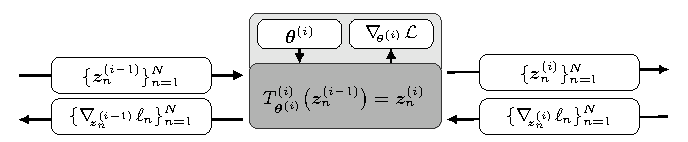
\includegraphics[width=\figureWidthPt pt]{../repos/backpack-paper/tex/paper/figs/backprop-modules/vanilla_backprop.pdf}};

  \newcommand{\relativeCoordinate}[2]{($(im.south west)!#1!(im.south east)+(im.south west)!#2!(im.north west)-(im.south west)$)}

  % bottom left
  \node [rectangle, fill=white, draw=none, inner sep=0pt, minimum height =
  0.04*\figureWidthPt pt, minimum width = 0.18*\figureWidthPt pt, anchor=center]
  at \relativeCoordinate{0.19}{0.18} {$\{ \grad{\vz_n^{(l-1)}}\ell_n \}_n$};

  % top left
  \node [rectangle, fill=white, draw=none, inner sep=0pt, minimum height =
  0.04*\figureWidthPt pt, minimum width = 0.18*\figureWidthPt pt, anchor=center]
  at \relativeCoordinate{0.19}{0.47} {$\{ \vz_n^{(l-1)}\}_n$};

  % bottom right
  \node [rectangle, fill=white, draw=none, inner sep=0pt, minimum height =
  0.04*\figureWidthPt pt, minimum width = 0.18*\figureWidthPt pt, anchor=center]
  at \relativeCoordinate{0.81}{0.18} {$\{ \grad{\vz_n^{(l)}}\ell_n \}_n$};

  % top right
  \node [rectangle, fill=white, draw=none, inner sep=0pt, minimum height =
  0.04*\figureWidthPt pt, minimum width = 0.18*\figureWidthPt pt, anchor=center]
  at \relativeCoordinate{0.81}{0.49} {$\{ \vz_n^{(l)}\}_n$};

  % center left
  \node [rectangle, fill=white, draw=none, inner sep=0pt, minimum height =
  0.035*\figureWidthPt pt, minimum width = 0.1*\figureWidthPt pt, anchor=center]
  at \relativeCoordinate{0.435}{0.76} {$\vtheta^{(l)}$};

  % center right
  \node [rectangle, fill=white, draw=none, inner sep=0pt, minimum height =
  0.035*\figureWidthPt pt, minimum width = 0.1*\figureWidthPt pt, anchor=center]
  at \relativeCoordinate{0.5685}{0.76} {$\grad{\vtheta^{(l)}}\gL$};

  % module
  \node [rectangle, fill=lightGray, draw=none, inner sep=0pt, minimum height =
  0.07*\figureWidthPt pt, minimum width = 0.25*\figureWidthPt pt, anchor=center]
  at \relativeCoordinate{0.5}{0.33} {$f_{\vtheta^{(l)}}^{(l)}$};
\end{tikzpicture}
%%% Local Variables:
%%% mode: latex
%%% TeX-master: "../../thesis"
%%% End:

  \tikzexternaldisable%
  \caption{\textbf{Schematic representation of the standard backpropagation
      pass} for module $l$ with $N$
    samples.}\label{backpack::fig:backprop-gradient}
\end{figure}

For second-order quantities, we rely on the work of
\citet{mizutani2008secondorder} and \citet{dangel2020modular}, who showed that a
scheme similar to \Cref{backpack::eq:backprop_gradient} exists for the
\emph{block diagonal} of the Hessian. A block \wrt the parameters of
a module, $\gradsquared{\vtheta^{(l)}}\ell_n(\vtheta)$, can be obtained by the
recursion
\begin{equation}
  \begin{split}
    \gradsquared{\vtheta^{(l)}}\ell_n(\vtheta)
    &=
    {\left(\jac_{\vtheta^{(l)}} \vz_n^{(l)}\right)}^\top
    \gradsquared{\vz_n^{(l)}}\ell_n(\vtheta)
    \left(\jac_{\vtheta^{(l)}} \vz_n^{(l)}\right)
    \\
    &\phantom{=}\
    + \sum_j
    \left(\gradsquared{\vtheta^{(l)}} {\left[\vz_n^{(l)}\right]}_j\right)
    {\left[ \grad{\vz_n^{(l)}}\ell_n(\vtheta) \right]}_j\equationPunctuation{.}
  \end{split}
  \label{backpack::eq:backprop_hessian}
\end{equation}
A similar relation holds for the module's output Hessian
$\gradsquared{\vz_n^{(l)}} \ell_n(\vtheta)$.

Both backpropagations of
\Cref{backpack::eq:backprop_gradient,backpack::eq:backprop_hessian} hinge on the
multiplication by Jacobians to both vectors and matrices. However, the design of
AD limits the application of Jacobians to vectors only. This prohibits the
exploitation of vectorization in the matrix case, which is needed for
second-order information. The lacking flexibility of Jacobians is one motivation
for our work. Since all quantities needed to compute statistics of the
derivatives are already computed during the backward pass, another motivation is
to provide access to them at minor overhead.

\subsection{First-order Extensions}
As the principal first-order extension, consider computing the \emph{per-sample}
gradients in a batch of size $N$. These individual gradients are implicitly
computed during a traditional backward pass because the batch gradient is their
sum, but they are not directly accessible. The naïve way to compute $N$
individual gradients is to do $N$ separate forward and backward passes, This
(inefficiently) replaces every matrix-matrix multiplication by $N$ matrix-vector
multiplications. \BackPACK batches computations to obtain large efficiency
gains, as illustrated by
\Cref{backpack::fig:bench-individual-gradients}\sidenote{%
  The latest developments in ML libraries have lead to more efficient
  alternatives than the for-loop. \pytorch 1.11.0 (released on March 10, 2022)
  introduced an \inlinecode{is\_grads\_batched} argument in the API of
  the
  \href{https://pytorch.org/docs/1.11/generated/torch.autograd.grad.html}{\inlinecode{grad}}
  function of
  its \href{https://pytorch.org/docs/1.11/autograd.html}{\inlinecode{autograd}}
  library, which allows to compute multiple VJPs in parallel. This reflects the
  importance of the feature.}.

\begin{figure}
  \centering
  \pgfkeys{/pgfplots/BackPACKBenchBarplot/.style={
    width=1.02\linewidth,
    height=0.5\linewidth,
    grid=major,
    grid style = {dashed},
    every axis plot/.append style={line width = 1.5pt},
    tick pos = left,
    xtick align = outside,
    ytick align = inside,
    xmajorticks = true,
    ymajorticks = true,
    ylabel near ticks,
    xlabel near ticks,
    xticklabel style = {font = \footnotesize},
    xlabel style = {font = \footnotesize},
    axis line style = {black},
    yticklabel style = {font = \footnotesize},
    ylabel style = {font = \footnotesize},
    title style = {font = \footnotesize, inner ysep = 0ex},
    grid = major,
    grid style = {dashed},
    legend cell align = left,
    legend style = {
      fill opacity = 0.7,
      text opacity = 1,
      font = \footnotesize,
      legend columns = 4,
      legend cell align={left},
      legend image post style={opacity = 1, yscale = 1.1, line width=-1pt},
      column sep=0.25cm,
    },
  }
}

%%% Local Variables:
%%% mode: latex
%%% TeX-master: "../../thesis"
%%% End:

  \pgfkeys{/pgfplots/zmystyle/.style={
      BackPACKBenchBarplot
    }
  }
  \tikzexternalenable%
  % This file was created by tikzplotlib v0.9.7.
\begin{tikzpicture}

\definecolor{color0}{rgb}{0.211764705882353,0.294117647058824,0.603921568627451}
\definecolor{color1}{rgb}{0.431372549019608,0.650980392156863,0.803921568627451}
\definecolor{color2}{rgb}{0.76078431372549,0.894117647058824,0.937254901960784}

\begin{axis}[
legend cell align={left},
legend style={fill opacity=0.8, draw opacity=1, text opacity=1, draw=white!80!black},
tick align=outside,
tick pos=left,
title={Batch gradients},
x grid style={white!69.0196078431373!black},
xmin=-0.5125, xmax=2.5125,
xtick style={color=black},
xtick={0,1,2},
xticklabels={For-loop,BackPACK,Gradient
(Ref.)},
y grid style={white!69.0196078431373!black},
ylabel={Time [ms]},
ymin=0, ymax=715.401721642411,
ytick style={color=black},
zmystyle
]
\draw[draw=none,fill=white!20!black] (axis cs:1.625,0) rectangle (axis cs:1.875,22.247069500736);
\draw[draw=none,fill=color0] (axis cs:-0.375,0) rectangle (axis cs:-0.125,190.67248400097);
\addlegendimage{ybar,ybar legend,draw=none,fill=color0};
\addlegendentry{Batch size 64}

\draw[draw=none,fill=color0] (axis cs:0.625,0) rectangle (axis cs:0.875,30.771913996432);
\draw[draw=none,fill=white!40!black] (axis cs:1.875,0) rectangle (axis cs:2.125,40.6486490028328);
\draw[draw=none,fill=color1] (axis cs:-0.125,0) rectangle (axis cs:0.125,367.899422002665);
\addlegendimage{ybar,ybar legend,draw=none,fill=color1};
\addlegendentry{                 128}

\draw[draw=none,fill=color1] (axis cs:0.875,0) rectangle (axis cs:1.125,57.7847249951446);
\draw[draw=none,fill=color2] (axis cs:0.125,0) rectangle (axis cs:0.375,681.334972992772);
\addlegendimage{ybar,ybar legend,draw=none,fill=color2};
\addlegendentry{                 256}

\draw[draw=none,fill=color2] (axis cs:1.125,0) rectangle (axis cs:1.375,96.5649990030215);
\draw[draw=none,fill=white!60!black] (axis cs:2.125,0) rectangle (axis cs:2.375,79.2037880019052);
\addplot [semithick, white!20!black, opacity=0.4, forget plot]
table {%
-0.5125 22.247069500736
2.5125 22.247069500736
};
\addplot [semithick, white!40!black, opacity=0.4, forget plot]
table {%
-0.5125 40.6486490028329
2.5125 40.6486490028329
};
\addplot [semithick, white!60!black, opacity=0.4, forget plot]
table {%
-0.5125 79.2037880019052
2.5125 79.2037880019052
};
\end{axis}

\end{tikzpicture}

  \tikzexternaldisable%
  \caption{\textbf{Computing individual gradients in a batch using a for-loop
      (\ie one individual forward and backward pass per sample) or using
      vectorized operations with \BackPACK.} The plot shows computation time,
    comparing to a traditional gradient computation, on the \CIFARTENNET%
    network (see \Cref{backpack::sec:experiments}) for the \CIFARTEN%
    dataset \citep{schneider2019deepobs}.
  }\label{backpack::fig:bench-individual-gradients}
\end{figure}

As the quantities necessary to compute the individual gradients are already
propagated through the computation graph, we can reuse them by inserting code in
the standard backward pass. With access to this information, before it is
cleared for memory efficiency, \BackPACK%
computes the Jacobian-multiplications
for each sample
\begin{equation}
  {\left\{
      \grad{\vtheta^{(l)}} \ell_n(\vtheta)
    \right\}}_{n=1}^N
  =
  {\left\{
      {\left(\jac_{\vtheta^{(l)}} \vz^{(l)}_n\right)}^\top \grad{\vz_n^{(l)}} \ell_n(\vtheta)
    \right\}}_{n=1}^N\equationPunctuation{,}
\end{equation}
without summing the result---see \Cref{backpack::fig:first-order-extraction} for
a schematic representation. This duplicates some of the computation performed by
the backpropagation, as the Jacobian is applied twice (once by \PyTorch%
and \BackPACK%
with and without summation over the samples, respectively). However, the
associated overhead is small compared to the for-loop approach: the major
computational cost arises from the propagation of information required for each
layer, rather than the formation of the gradient \emph{within} each layer.

This scheme for individual gradient computation is the basis for all first-order
extensions. In this direct form, however, it is expensive in memory: if the
model is $D$-dimensional, storing $\gO(ND)$ elements is prohibitive for large
batches. For the variance, 2\textsuperscript{nd} moment and $L_2$ norm,
\BackPACK%
takes advantage of the Jacobian's structure to directly compute them without
forming the individual gradient, reducing memory overhead. See
\Cref{backpack::app:first-order-extensions} for details.

\begin{figure}[!t]
  \centering
  \tikzexternalenable%
  \begin{tikzpicture}
  \definecolor{lightBlue}{HTML}{d1e5f0}
  \definecolor{lightGray}{HTML}{b3b3b3}
  \pgfmathsetmacro{\figureWidthPt}{\linewidth}

  \node (im) [inner sep=0pt] {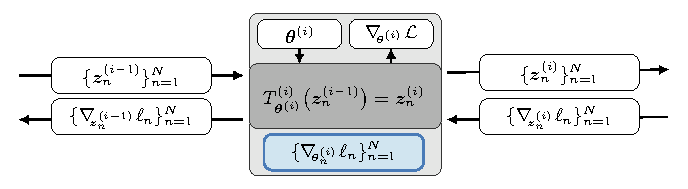
\includegraphics[width=\figureWidthPt pt]{../repos/backpack-paper/tex/paper/figs/backprop-modules/indiv_grad.pdf}};

  \newcommand{\relativeCoordinate}[2]{($(im.south west)!#1!(im.south east)+(im.south west)!#2!(im.north west)-(im.south west)$)}

  % bottom left
  \node [rectangle, fill=white, draw=none, inner sep=0pt, minimum height =
  0.04*\figureWidthPt pt, minimum width = 0.18*\figureWidthPt pt, anchor=center]
  at \relativeCoordinate{0.19}{0.385} {$\{ \grad{\vz_n^{(l-1)}}\ell_n \}_n$};

  % top left
  \node [rectangle, fill=white, draw=none, inner sep=0pt, minimum height =
  0.04*\figureWidthPt pt, minimum width = 0.18*\figureWidthPt pt, anchor=center]
  at \relativeCoordinate{0.19}{0.6} {$\{ \vz_n^{(l-1)}\}_n$};

  % bottom right
  \node [rectangle, fill=white, draw=none, inner sep=0pt, minimum height =
  0.04*\figureWidthPt pt, minimum width = 0.18*\figureWidthPt pt, anchor=center]
  at \relativeCoordinate{0.81}{0.385} {$\{ \grad{\vz_n^{(l)}}\ell_n \}_n$};

  % top right
  \node [rectangle, fill=white, draw=none, inner sep=0pt, minimum height =
  0.04*\figureWidthPt pt, minimum width = 0.18*\figureWidthPt pt, anchor=center]
  at \relativeCoordinate{0.81}{0.615} {$\{ \vz_n^{(l)}\}_n$};

  % center left
  \node [rectangle, fill=white, draw=none, inner sep=0pt, minimum height =
  0.03*\figureWidthPt pt, minimum width = 0.1*\figureWidthPt pt, anchor=center]
  at \relativeCoordinate{0.435}{0.82} {$\vtheta^{(l)}$};

  % center right
  \node [rectangle, fill=white, draw=none, inner sep=0pt, minimum height =
  0.03*\figureWidthPt pt, minimum width = 0.1*\figureWidthPt pt, anchor=center]
  at \relativeCoordinate{0.5685}{0.82} {$\grad{\vtheta^{(l)}}\gL$};

  % module
  \node [rectangle, fill=lightGray, draw=none, inner sep=0pt, minimum height =
  0.05*\figureWidthPt pt, minimum width = 0.25*\figureWidthPt pt, anchor=center]
  at \relativeCoordinate{0.5}{0.49} {$f_{\vtheta^{(l)}}^{(l)}$};

  % center bottom
  \node [rectangle, fill=lightBlue, draw=none, inner sep=0pt, minimum height =
  0.04*\figureWidthPt pt, minimum width = 0.2*\figureWidthPt pt, anchor=center]
  at \relativeCoordinate{0.5}{0.195} {$\{ \grad{\vtheta^{(l)}} \ell_n\}_n$};
\end{tikzpicture}
%%% Local Variables:
%%% mode: latex
%%% TeX-master: "../../thesis"
%%% End:

  \tikzexternaldisable%
  \caption{\textbf{Schematic representation of the individual gradients'
      extraction in addition to the standard backward pass} at the $l$th module
      for $N$ samples.}\label{backpack::fig:first-order-extraction}
\end{figure}

\subsection{Second-order Extensions}\label{backpack::sec:backpack-second-order}
Second-order extensions require propagation of more information through the
graph. %
\marginnote[*-20]{
  \begin{example}[\textbf{Symmetric decomposition of the softmax cross-entropy loss
    Hessian~\cite{papyan2019measurements}}]\label{ex:backpack::symmetricDecompositionCE}
  Consider the softmax cross-entropy loss
  (\Cref{eq:background::softmaxCrossEntropyLoss}) Hessian from Table
  \Cref{hbp::table:backpropEquations}. Its symmetric decomposition $\mS \in
  \sR^{C\times C}$ is
    \begin{align}
      \label{eq:backpack::sqrtCrossEntropyLoss}
      \begin{split}
        \mS
        &=
          \left(
          \mI - \vp\,\vone^{\top}
          \right)
          \diag\left( \sqrt{\vp} \right)
        \\
        &=
          \diag\left( \sqrt{\vp} \right)
          -
          \vp \sqrt{\vp}^{\top}\,,
      \end{split}
    \end{align}
    where $\sqrt{\vp(\vf)} = {\vp(\vf)}^{\odot \nicefrac{1}{2}}$. It satisfies
    $\gradsquared{\vf}\ell(\vf, \vy) = \mS \mS^{\top}$,
    \begin{align*}
      \mS \mS^{\top}
      &=
        \left[
        \diag\left( \sqrt{\vp} \right)
        -
        \vp \sqrt{\vp}^{\top}\,
        \right]
      \\
      &\phantom{= \ }
        \left[
        \diag\left( \sqrt{\vp} \right)
        -
        \sqrt{\vp} \vp^{\top}\,
        \right]
      \\
      &=
        \diag\left( \vp \right)
        - 2 \vp \vp^{\top}
        + \vp \sqrt{\vp}^{\top}
        \sqrt{\vp} \vp^{\top}
      \\
      &=
        \diag\left( \vp \right)
        - \vp \vp^{\top}\,,
    \end{align*}
    using that $\vp$'s elements sum to one, \ie $\sqrt{\vp}^{\top}\sqrt{\vp} =
    1$. This is the expression from \Cref{hbp::table:backpropEquations}.
  \end{example}
}%
As an example, we will focus on the \GGN matrix
\citep{schraudolph2002fast}. It is guaranteed to be PSD and is a reasonable
approximation of the Hessian near the minimum, which motivates its use in
approximate second-order methods. For popular loss functions, it coincides with
the Fisher information matrix used in natural gradient methods
\citep{amari1998natural}; for a more in depth discussion of the equivalence, see
\Cref{sec:background::naturalGradientDescent} and the reviews of
\citet{martens2014new} and \citet{kunstner2019limitations}. For an objective
function that can be written as the composition of a loss function $\ell$ and a
model $f_{\vtheta}$, such as \Cref{backpack::eq:objective}, the \GGN%
of $\nicefrac{1}{N} \sum_n \ell(f_{\vtheta}(\vx_n), \vy_n)$ is
\begin{equation}
  \label{backpack::eq:main-ggn}
  \mG(\vtheta) =
  \frac{1}{N} \sum_n
  {\left(\jac_\vtheta \vf_n \right)}^\top
  \gradsquared{\vf_n} \ell(\vf_n, \vy_n) \:
  \left(\jac_\vtheta \vf_n\right)\equationPunctuation{.}
\end{equation}
\marginnote[*-10]{%
  \begin{example}[\textbf{\mc approximation of the softmax-cross entropy loss
    Hessian}]\label{ex:backpack::symmetricMCDecompositionCE} Consider the softmax
  cross-entropy loss (\Cref{eq:background::softmaxCrossEntropyLoss}) Hessian
  from \Cref{hbp::table:backpropEquations}. An \mc approximation of the
  symmetric decomposition (\Cref{eq:backpack::sqrtCrossEntropyLoss}) is
  constructed by the vectors
    \begin{align}
      \label{equ:backpack::sqrtMCVectorsCrossEntropyLoss}
      \vstilde = \vytilde(c) - \vp(\vf)
    \end{align}
    with $\vytilde(c) = \onehot(c)$ and $c$ drawn from a categorical
    distribution implied by the softmax-probabilities, $c \sim \Cat(c;
    \vp(\vf))$. The random vector $\vytilde$ satisfies $\E_{c}\left[ \vytilde
    \right] = \vp(\vf)$ and $\E_{c}\left[ \vytilde \vytilde^{\top} \right] =
    \diag[\vp(\vf)]$. With these properties, we can show
    $\E_{\vstilde}\left[\vstilde\vstilde^{\top}\right] = \gradsquared{\vf}\ell$,
    \ie%
    the expected outer product of
    \Cref{equ:backpack::sqrtMCVectorsCrossEntropyLoss} is the Hessian,
    \begin{align*}
      \E_{\vstilde} \left[\vstilde \vstilde^{\top}\right]
      &=
        \E_{c}[ \vytilde \vytilde^{\top} ]
        - \E_{c}[ \vytilde]  \vp^{\top}
      \\
      &\phantom{= \,}
        -  \vp \E_{c}[\vytilde^{\top} ]
        + \vp \vp^{\top}
      % \\
      % &=
      %   \diag(\vp) - 2 \vp \vp^{\top} + \vp\vp^{\top}
      \\
      &=
        \diag(\vp) - \vp \vp^{\top}\,.
    \end{align*}
    Instead of using the $C \times C$ matrix square root $\mS$, we can draw $M <
    C$ samples $c_1, \dots, c_M$ and stack their $\vstilde$-vectors into a
    smaller $C \times M $ matrix
    \begin{align}
      \mStilde
      =
      \frac{1}{\sqrt{M}}
      \begin{pmatrix}
        \vstilde(c_1)\  \dots\  \vstilde(c_M)
      \end{pmatrix}
    \end{align}
    that approximates \Cref{eq:backpack::sqrtCrossEntropyLoss},
    \begin{align*}
      \mStilde \mStilde^{\top}
      &=
        \frac{1}{M}
        \sum_{i=1}^{M}
        \vstilde(c_i)
        {\vstilde(c_i)}^{\top}
      \\
      &\approx \E_{\vstilde}\left[ \vstilde \vstilde^{\top}\right]
        = \mS \mS^{\top}\,,
    \end{align*}
    using less memory. From the connection between Fisher and Hessian,
    \Cref{equ:backpack::sqrtMCVectorsCrossEntropyLoss} are `would-be gradients'
    under targets sampled from the model's likelihood, \ie%
    $\vstilde^{\top} = \jac_{\vf}\ell(\vf, \vytilde)$ with $\vytilde \sim
    q(\giventhat{\cdot}{\vf})$ and the Jacobian from
    \Cref{tab:background::Jacobians}.
  \end{example}
}%
The full matrix is too large to compute and store. Current approaches focus on
its diagonal blocks, where each block corresponds to a layer in the network.
Every block itself is further approximated, for example using a Kronecker
factorization. The approach used by \BackPACK%
for their computation is a refinement of the \emph{Hessian Backpropagation
  equations} of \citet{dangel2020modular}. It relies on two insights: firstly,
the computational bottleneck in the \ggn's computation is the multiplication
with the Jacobian of the network, $\jac_\vtheta \vf_n$, while the network output
Hessian is easy to compute for most popular loss functions. Secondly, it is not
necessary to compute and store each of the $N$ $D \times D$ matrices for a
network with $D$ parameters, as \Cref{backpack::eq:main-ggn} is a quadratic
expression. Given a symmetric factorization $\mS_n$ of the Hessian,
$\mS_n\mS_n^\top = \gradsquared{\vf_n} \ell(\vf_n, \vy_n)$ (\eg
\Cref{ex:backpack::symmetricDecompositionCE}), it is sufficient to compute
${(\jac_\vtheta \vf_n)}^\top \mS_n$ and square the result. A network output is
typically small compared to its inner layers; networks on \CIFARHUN%
need $C=100$ class outputs but could use convolutional layers with more than
100,000 parameters.

The factorization leads to a $D \times C$ matrix, which makes it possible to
efficiently compute \GGN%
block diagonals. Also, the computation is very similar to that of a gradient,
which computes ${(\jac_\vtheta \vf_n)}^\top \grad{\vf_n} \ell_n$. A module
$f^{(l)}_{\vtheta^{(l)}}$ receives the symmetric factorization of the \GGN%
\wrt its output, $\vz^{(l)}_n$, and multiplies it with the Jacobians
\wrt the parameters $\vtheta^{(l)}$ and inputs $\vz^{(l-1)}_n$ to
produce a symmetric factorization of the \GGN%
\wrt the parameters and inputs, as shown in
\Cref{backpack::fig:second-order-pass}.

\begin{figure}[!t]
  \centering
  \tikzexternalenable%
  \begin{tikzpicture}
  \definecolor{lightBlue}{HTML}{d1e5f0}
  \definecolor{lightGray}{HTML}{b3b3b3}
  \pgfmathsetmacro{\figureWidthPt}{\linewidth}

  \node (im) [inner sep=0pt] {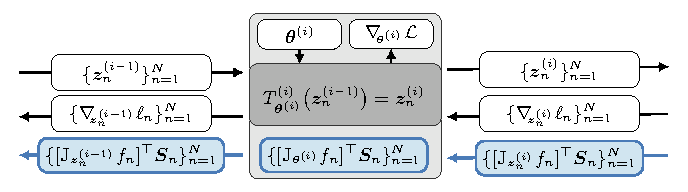
\includegraphics[width=\figureWidthPt pt]{../repos/backpack-paper/tex/paper/figs/backprop-modules/second_order.pdf}};

  \newcommand{\relativeCoordinate}[2]{($(im.south west)!#1!(im.south east)+(im.south west)!#2!(im.north west)-(im.south west)$)}

  % bottom left
  \node [rectangle, fill=lightBlue, draw=none, inner sep=0pt, minimum height =
  0.04*\figureWidthPt pt, minimum width = 0.245*\figureWidthPt pt, anchor=center]
  at \relativeCoordinate{0.19}{0.195} {$\{ {(\jac_{\vz_n^{(l-1)}} \vf_n)}^{\top} \mS_n \}_n$};

  % center left
  \node [rectangle, fill=white, draw=none, inner sep=0pt, minimum height =
  0.04*\figureWidthPt pt, minimum width = 0.18*\figureWidthPt pt, anchor=center]
  at \relativeCoordinate{0.19}{0.41} {$\{ \grad{\vz_n^{(l-1)}}\ell_n \}_n$};

  % top left
  \node [rectangle, fill=white, draw=none, inner sep=0pt, minimum height =
  0.04*\figureWidthPt pt, minimum width = 0.18*\figureWidthPt pt, anchor=center]
  at \relativeCoordinate{0.19}{0.625} {$\{ \vz_n^{(l-1)}\}_n$};

  % bottom right
  \node [rectangle, fill=lightBlue, draw=none, inner sep=0pt, minimum height =
  0.04*\figureWidthPt pt, minimum width = 0.225*\figureWidthPt pt, anchor=center]
  at \relativeCoordinate{0.814}{0.18} {$\{ {(\jac_{\vz_n^{(l)}} \vf_n)}^{\top} \mS_n \}_n$};

  % center right
  \node [rectangle, fill=white, draw=none, inner sep=0pt, minimum height =
  0.04*\figureWidthPt pt, minimum width = 0.18*\figureWidthPt pt, anchor=center]
  at \relativeCoordinate{0.81}{0.41} {$\{ \grad{\vz_n^{(l)}}\ell_n \}_n$};

  % top right
  \node [rectangle, fill=white, draw=none, inner sep=0pt, minimum height =
  0.04*\figureWidthPt pt, minimum width = 0.18*\figureWidthPt pt, anchor=center]
  at \relativeCoordinate{0.81}{0.64} {$\{ \vz_n^{(l)}\}_n$};

  % center left
  \node [rectangle, fill=white, draw=none, inner sep=0pt, minimum height =
  0.03*\figureWidthPt pt, minimum width = 0.1*\figureWidthPt pt, anchor=center]
  at \relativeCoordinate{0.435}{0.82} {$\vtheta^{(l)}$};

  % center right
  \node [rectangle, fill=white, draw=none, inner sep=0pt, minimum height =
  0.03*\figureWidthPt pt, minimum width = 0.1*\figureWidthPt pt, anchor=center]
  at \relativeCoordinate{0.5685}{0.82} {$\grad{\vtheta^{(l)}}\gL$};

  % module
  \node [rectangle, fill=lightGray, draw=none, inner sep=0pt, minimum height =
  0.05*\figureWidthPt pt, minimum width = 0.25*\figureWidthPt pt, anchor=center]
  at \relativeCoordinate{0.5}{0.49} {$\vf_{\vtheta^{(l)}}^{(l)}$};

  % center bottom
  \node [rectangle, fill=lightBlue, draw=none, inner sep=0pt, minimum height =
  0.04*\figureWidthPt pt, minimum width = 0.22*\figureWidthPt pt, anchor=center]
  at \relativeCoordinate{0.5}{0.195} {$\{ {(\jac_{\vtheta^{(l)}} \vf_n)}^{\top} \mS_n \}_n$};
\end{tikzpicture}
%%% Local Variables:
%%% mode: latex
%%% TeX-master: "../../thesis"
%%% End:

  \tikzexternaldisable%
  \caption{\textbf{Schematic of the additional backward pass} to compute a
    symmetric factorization of the \GGN,
    \begin{align*}
      \mG(\vtheta) = \frac{1}{N} \sum_n {\left(\jac_{\vtheta} \vf_n\right)}^\top \mS_n \mS_n^\top
      \left(\jac_{\vtheta} \vf_n\right)
    \end{align*}
    alongside the gradient at the $l$th module, for $N$ samples.
  }\label{backpack::fig:second-order-pass}
\end{figure}

This propagation serves as the basis of the second-order extensions. If the full
symmetric factorization is not wanted, for memory reasons, it is possible to
extract more specific information such as the diagonal. If $\mB$ is the
symmetric factorization for a \GGN%
block, the diagonal can be computed as $[\diag(\mB\mB^\top)]_{i} =
{[\mB\mB^\top]}_{i,i} = \sum_j {[\mB]}_{i,j}^2$.

This framework can be used to extract the main Kronecker factorizations of the
\GGN, \KFAC%
and \KFLR, which we extend to convolution using the approach of
\citet{grosse2016kronecker}. The important difference between the two methods is
the initial matrix factorization $\mS_n$. Using a full symmetric factorization
of the initial Hessian, $\mS_n\mS_n^\top = \gradsquared{\vf_n}\ell_n$, yields
the \KFLR%
approximation. \KFAC%
uses an \MC approximation by sampling a vector $\vs_n$ such that
$\mathbb{E}_{\vs_n}[\vs_n\vs_n^\top] = \gradsquared{\vf_n} \ell_n$ (see
\Cref{ex:backpack::symmetricMCDecompositionCE}). \KFLR%
is therefore more precise but more expensive than \KFAC, especially for networks
with high-dimensional outputs, which is reflected in our benchmark on \CIFARHUN%
in \Cref{backpack::sec:benchmark}. The technical details on how Kronecker
factors are extracted and information is propagated for second-order \BackPACK%
extensions are documented in \Cref{backpack::app:second-order-extensions}.

%%% Local Variables:
%%% mode: latex
%%% TeX-master: "../thesis"
%%% End:


\section{Evaluation \& Benchmarks}\label{backpack::sec:benchmark}
We benchmark the overhead of \BackPACK %
on \CIFARTEN and \CIFARHUN, using the \CIFARTENNET network and the \ALLCNNC
network of \citet{springenberg2015striving} provided by \DeepOBS
\citep{schneider2019deepobs}\sidenote{\CIFARTENNET is a sequence of three
  convolutions and three dense linear layers with 895,210 parameters. \ALLCNNC
  is a sequence of nine convolutions with 1,387,108 parameters.}.
\Cref{backpack::fig:benchmark-all} shows the results.

For first-order extensions, the computation of individual gradients from a
mini-batch adds noticeable overhead due to the additional memory requirements to
store them. But more specific quantities such as the $L_2$ norm,
2\textsuperscript{nd} moment and variance can be extracted efficiently.
Regarding second-order extensions, the \ggn computation can be expensive for
nets with large outputs like \CIFAR{100}, regardless of the approximation being
diagonal of Kronecker-factored. Thankfully, the \MC approximation used by \KFAC,
which we also implement for a diagonal approximation, can be computed at minimal
overhead---much less than two backward passes. This last point is encouraging,
as our optimization experiment in \Cref{backpack::sec:experiments} suggest that
this approximation is reasonably accurate.

%%% Local Variables:
%%% mode: latex
%%% TeX-master: "../thesis"
%%% End:


\section{Experiments}\label{backpack::sec:experiments}
To illustrate the utility of \BackPACK, we implement preconditioned gradient
descent optimizers using diagonal and Kronecker approximations of the \GGN. To
our knowledge, and despite their apparent simplicity, results using diagonal
approximations or the naïve damping update rule we chose have not been reported
in publications so far. However, this section is not meant to introduce a
bona-fide new optimizer. Our goal is to show that \BackPACK can enable research
of this kind. The update rule we implement uses a curvature matrix
$\mC(\vtheta_t^{(l)})$, which could be a diagonal or Kronecker factorization of
the \GGN blocks, and a damping parameter $\lambda$ to precondition the gradient:
\begin{equation}
  \label{backpack::eq:update_rule}
  \vtheta_{t+1}^{(l)}
  =
  \vtheta_t^{(l)} - \eta \left(\mC(\vtheta_t^{(l)}) + \lambda \mI\right)^{-1}
  \grad{\vtheta_t^{(l)}}\Loss(\vtheta_t^{(l)})\equationPunctuation{,}
  \qquad l = 1,\dots, L\equationPunctuation{.}
\end{equation}
We run the update rule with the following approximations of the generalized
Gauss-Newton: the exact diagonal (\DiagGGN) and an \MC estimate (\DiagGGNMC),
and the Kronecker factorizations \KFAC \citep{martens2015optimizing}, \KFLR and
\KFRA\sidenote{ \KFRA was not originally designed for convolutions; we extend it
  using the Kronecker factorization of \citet{grosse2016kronecker}. While it can
  be computed for small networks on \MNIST, which we report in
  \Cref{backpack::app:additional-results}, the approximate backward pass of
  \KFRA does not seem to scale to large convolution layers. }
\citep{botev2017practical}.%
The inversion required by the update rule is straightforward for the diagonal
curvature. For the Kronecker-factored quantities, we use the approximation
introduced by \cite{martens2015optimizing} (see
\Cref{backpack::app:update_rule_details}).

\begin{figure*}[!t]
  \centering
  \pgfkeys{/pgfplots/BackPACKBenchBarplot/.style={
    width=1.02\linewidth,
    height=0.5\linewidth,
    grid=major,
    grid style = {dashed},
    every axis plot/.append style={line width = 1.5pt},
    tick pos = left,
    xtick align = outside,
    ytick align = inside,
    xmajorticks = true,
    ymajorticks = true,
    ylabel near ticks,
    xlabel near ticks,
    xticklabel style = {font = \footnotesize},
    xlabel style = {font = \footnotesize},
    axis line style = {black},
    yticklabel style = {font = \footnotesize},
    ylabel style = {font = \footnotesize},
    title style = {font = \footnotesize, inner ysep = 0ex},
    grid = major,
    grid style = {dashed},
    legend cell align = left,
    legend style = {
      fill opacity = 0.7,
      text opacity = 1,
      font = \footnotesize,
      legend columns = 4,
      legend cell align={left},
      legend image post style={opacity = 1, yscale = 1.1, line width=-1pt},
      column sep=0.25cm,
    },
  }
}

%%% Local Variables:
%%% mode: latex
%%% TeX-master: "../../thesis"
%%% End:

  \begin{subfigure}[t]{1.0\linewidth}
    \centering
    \caption{\threecthreed, \cifarten}\label{backpack::subfig:benchmark-all1}
    \vspace{-1ex}
    \pgfkeys{/pgfplots/zmystyle/.style={
        BackPACKBenchBarplot,
        height = 0.35\linewidth,
        title = \empty,
      }
    }
    \tikzexternalenable
    % This file was created by tikzplotlib v0.9.7.
\begin{tikzpicture}

\definecolor{color0}{rgb}{0.211764705882353,0.294117647058824,0.603921568627451}
\definecolor{color1}{rgb}{0.431372549019608,0.650980392156863,0.803921568627451}
\definecolor{color2}{rgb}{0.76078431372549,0.894117647058824,0.937254901960784}

\begin{axis}[
legend cell align={left},
legend columns=4,
legend style={fill opacity=0.8, draw opacity=1, text opacity=1, at={(0.03,0.97)}, anchor=north west, draw=white!80!black},
tick align=outside,
tick pos=left,
title={3C3D on CIFAR10},
x grid style={white!69.0196078431373!black},
xmin=-0.5, xmax=7.5,
xtick style={color=black},
xtick={0,1,2,3,4,5,6,7},
xticklabels={
Grad (ref.),2nd Moment,
Batch L2,DiagGGN-MC,
KFAC,Indiv. Grad,
KFLR,DiagGGN},
y grid style={white!69.0196078431373!black},
ylabel={Time [ms]},
ymin=0, ymax=50,
ytick style={color=black},
zmystyle
]
\draw[draw=none,fill=white!20!black] (axis cs:-0.375,0) rectangle (axis cs:-0.125,15.0664545000154);
\draw[draw=none,fill=color0] (axis cs:0.625,0) rectangle (axis cs:0.875,14.395405000073);
\addlegendimage{ybar,ybar legend,draw=none,fill=color0};
\addlegendentry{Batch = 32}

\draw[draw=none,fill=color0] (axis cs:1.625,0) rectangle (axis cs:1.875,15.2878979999969);
\draw[draw=none,fill=color0] (axis cs:2.625,0) rectangle (axis cs:2.875,19.3677970000863);
\draw[draw=none,fill=color0] (axis cs:3.625,0) rectangle (axis cs:3.875,16.8086539999877);
\draw[draw=none,fill=color0] (axis cs:4.625,0) rectangle (axis cs:4.875,15.2265290000742);
\draw[draw=none,fill=color0] (axis cs:5.625,0) rectangle (axis cs:5.875,21.8555310000283);
\draw[draw=none,fill=color0] (axis cs:6.625,0) rectangle (axis cs:6.875,22.4338249999505);
\draw[draw=none,fill=white!40!black] (axis cs:-0.125,0) rectangle (axis cs:0.125,20.5737690000092);
\draw[draw=none,fill=color1] (axis cs:0.875,0) rectangle (axis cs:1.125,20.6966069999908);
\addlegendimage{ybar,ybar legend,draw=none,fill=color1};
\addlegendentry{48}

\draw[draw=none,fill=color1] (axis cs:1.875,0) rectangle (axis cs:2.125,20.9739174999868);
\draw[draw=none,fill=color1] (axis cs:2.875,0) rectangle (axis cs:3.125,25.4147299999659);
\draw[draw=none,fill=color1] (axis cs:3.875,0) rectangle (axis cs:4.125,22.383585);
\draw[draw=none,fill=color1] (axis cs:4.875,0) rectangle (axis cs:5.125,20.8398080000052);
\draw[draw=none,fill=color1] (axis cs:5.875,0) rectangle (axis cs:6.125,30.4188420000173);
\draw[draw=none,fill=color1] (axis cs:6.875,0) rectangle (axis cs:7.125,33.1303219999199);
\draw[draw=none,fill=white!60!black] (axis cs:0.125,0) rectangle (axis cs:0.375,26.3089910000645);
\draw[draw=none,fill=color2] (axis cs:1.125,0) rectangle (axis cs:1.375,26.2560775000225);
\addlegendimage{ybar,ybar legend,draw=none,fill=color2};
\addlegendentry{64}

\draw[draw=none,fill=color2] (axis cs:2.125,0) rectangle (axis cs:2.375,28.7451689999898);
\draw[draw=none,fill=color2] (axis cs:3.125,0) rectangle (axis cs:3.375,32.0420350000177);
\draw[draw=none,fill=color2] (axis cs:4.125,0) rectangle (axis cs:4.375,28.0495179999889);
\draw[draw=none,fill=color2] (axis cs:5.125,0) rectangle (axis cs:5.375,30.8939720000581);
\draw[draw=none,fill=color2] (axis cs:6.125,0) rectangle (axis cs:6.375,37.0278835000022);
\draw[draw=none,fill=color2] (axis cs:7.125,0) rectangle (axis cs:7.375,47.5826415000711);
\addplot [semithick, white!20!black, opacity=0.4, forget plot]
table {%
-0.5 15.0664545000154
7.5 15.0664545000154
};
\addplot [semithick, white!40!black, opacity=0.4, forget plot]
table {%
-0.5 20.5737690000092
7.5 20.5737690000092
};
\addplot [semithick, white!60!black, opacity=0.4, forget plot]
table {%
-0.5 26.3089910000645
7.5 26.3089910000645
};
\end{axis}

\end{tikzpicture}

    \tikzexternaldisable
  \end{subfigure}
  \begin{subfigure}[t]{1.0\linewidth}
    \centering
    \caption{\allcnnc, \cifarhun}\label{backpack::subfig:benchmark-all2}
    \vspace{-1ex}
    \pgfkeys{/pgfplots/zmystyle/.style={
        BackPACKBenchBarplot,
        height = 0.35\linewidth,
        ylabel = {Time [ms]},
        title = \empty,
      }
    }
    \tikzexternalenable
    \hspace{-1ex}% This file was created by tikzplotlib v0.9.7.
\begin{tikzpicture}

\definecolor{color0}{rgb}{0.211764705882353,0.294117647058824,0.603921568627451}
\definecolor{color1}{rgb}{0.431372549019608,0.650980392156863,0.803921568627451}
\definecolor{color2}{rgb}{0.76078431372549,0.894117647058824,0.937254901960784}

\begin{axis}[
legend cell align={left},
legend columns=4,
legend style={fill opacity=0.8, draw opacity=1, text opacity=1, at={(0.03,0.97)}, anchor=north west, draw=white!80!black},
tick align=outside,
tick pos=left,
title={All-CNN-C on CIFAR100},
x grid style={white!69.0196078431373!black},
xmin=-0.5, xmax=5.5,
xtick style={color=black},
xtick={0,1,2,3,4,5},
xticklabels={
Grad (ref.),2nd Moment,
Batch L2,DiagGGN-MC,
KFAC,Indiv. Grad},
y grid style={white!69.0196078431373!black},
ymin=0, ymax=113.550937500011,
ytick style={color=black},
zmystyle
]
\draw[draw=none,fill=white!20!black] (axis cs:-0.375,0) rectangle (axis cs:-0.125,17.0513680000113);
\draw[draw=none,fill=color0] (axis cs:0.625,0) rectangle (axis cs:0.875,23.2273660000146);
\addlegendimage{ybar,ybar legend,draw=none,fill=color0};
\addlegendentry{Batch = 32}

\draw[draw=none,fill=color0] (axis cs:1.625,0) rectangle (axis cs:1.875,29.9791224999808);
\draw[draw=none,fill=color0] (axis cs:2.625,0) rectangle (axis cs:2.875,27.1620119999625);
\draw[draw=none,fill=color0] (axis cs:3.625,0) rectangle (axis cs:3.875,38.6299799999961);
\draw[draw=none,fill=color0] (axis cs:4.625,0) rectangle (axis cs:4.875,55.4445244999897);
\draw[draw=none,fill=white!40!black] (axis cs:-0.125,0) rectangle (axis cs:0.125,23.4135965000064);
\draw[draw=none,fill=color1] (axis cs:0.875,0) rectangle (axis cs:1.125,32.411140000022);
\addlegendimage{ybar,ybar legend,draw=none,fill=color1};
\addlegendentry{48}

\draw[draw=none,fill=color1] (axis cs:1.875,0) rectangle (axis cs:2.125,39.3030079999335);
\draw[draw=none,fill=color1] (axis cs:2.875,0) rectangle (axis cs:3.125,38.0351860000019);
\draw[draw=none,fill=color1] (axis cs:3.875,0) rectangle (axis cs:4.125,53.98943900002);
\draw[draw=none,fill=color1] (axis cs:4.875,0) rectangle (axis cs:5.125,81.7799224999476);
\draw[draw=none,fill=white!60!black] (axis cs:0.125,0) rectangle (axis cs:0.375,30.1599859999442);
\draw[draw=none,fill=color2] (axis cs:1.125,0) rectangle (axis cs:1.375,41.9460425000011);
\addlegendimage{ybar,ybar legend,draw=none,fill=color2};
\addlegendentry{64}

\draw[draw=none,fill=color2] (axis cs:2.125,0) rectangle (axis cs:2.375,49.1684415000009);
\draw[draw=none,fill=color2] (axis cs:3.125,0) rectangle (axis cs:3.375,48.6743639999077);
\draw[draw=none,fill=color2] (axis cs:4.125,0) rectangle (axis cs:4.375,69.9318230000472);
\draw[draw=none,fill=color2] (axis cs:5.125,0) rectangle (axis cs:5.375,108.143750000011);
\addplot [semithick, white!20!black, opacity=0.4, forget plot]
table {%
-0.5 17.0513680000113
5.5 17.0513680000113
};
\addplot [semithick, white!40!black, opacity=0.4, forget plot]
table {%
-0.5 23.4135965000064
5.5 23.4135965000064
};
\addplot [semithick, white!60!black, opacity=0.4, forget plot]
table {%
-0.5 30.1599859999442
5.5 30.1599859999442
};
\end{axis}

\end{tikzpicture}

    \tikzexternaldisable
  \end{subfigure}
  \caption{ \textbf{Overhead benchmark for computing the gradient \emph{and}
      first- or second-order extensions on real networks, compared to just the
      gradient.} Most quantities add little overhead. \KFLR and \DiagGGN
    propagate 100$\times$ more information than \KFAC and \DiagGGNMC on
    \CIFAR{100} and are two orders of magnitude slower. We report benchmarks on
    those, and the Hessian's diagonal, in \Cref{backpack::app:benchmark}. }
  \label{backpack::fig:benchmark-all}
\end{figure*}


\begin{figure*}[!t]
  \centering
  \begin{subfigure}[t]{1.0\linewidth}
    \centering
    \caption{}\label{backpack::subfig:cifar1}
    \vspace{-5.5ex}
    \begin{center}\textbf{\footnotesize \CIFARTEN : \CIFARTENNET}\end{center}
    \tikzexternalenable
    \plotDifferentCurvatures{cifar10}{3c3d}{const}{final}{valid}{accuracies}
    \tikzexternaldisable
  \end{subfigure}
  \vspace{-2ex}
  \begin{subfigure}[t]{1.0\linewidth}
    \centering
    \caption{}\label{backpack::subfig:cifar2}
    \vspace{-5.5ex}
    \begin{center}\textbf{\footnotesize \CIFARHUN : \ALLCNNC}\end{center}
    \tikzexternalenable
    \plotDifferentCurvatures{cifar100}{allcnnc}{const}{final}{valid}{accuracies}
    \tikzexternaldisable
  \end{subfigure}
  \caption{\textbf{Median performance with shaded quartiles of the \DeepOBS
      benchmark} for \subfigref{backpack::subfig:cifar1} \CIFARTENNET (895,210
    parameters) on \CIFARTEN and \subfigref{backpack::subfig:cifar1} \ALLCNNC
    (1,387,108 parameters) on \CIFARHUN. Solid lines show \DeepOBS' baselines of
    momentum \SGD and Adam.}
  \label{backpack::fig:cifar}
\end{figure*}

These curvature estimates are tested for the training of deep neural networks by
running the corresponding optimizers on the main test problems of the
benchmarking suite \DeepOBS\sidenote{%
  \href{https://deepobs.github.io/}{\texttt{deepobs.github.io}}. We cannot run
  \BackPACK on all test problems in this benchmark due to the limitations
  outlined in \Cref{backpack::sec:theory-and-implementation}. Despite this
  limitation, we still run on models spanning a representative range of image
  classification problems. } \citep{schneider2019deepobs}. We use the setup
(batch size, number of training epochs) of \DeepOBS' baselines, and tune the
learning rate $\eta$ and damping parameter $\lambda$ with a grid search for
each optimizer (details in \Cref{backpack::app:grid-search}). The best
hyperparameter settings is chosen according to the final accuracy on a
validation set. We report the median and quartiles of the performance for ten
random seeds.

\Cref{backpack::subfig:cifar1} shows the results for the \CIFARTENNET network
trained on \CIFAR{10}. The optimizers that leverage Kronecker-factored curvature
approximations beat the baseline performance in terms of per-iteration progress
on the training loss, training and test accuracy. Using the same
hyperparameters, there is little difference between \KFAC and \KFLR, or \DiagGGN
and \DiagGGNMC. Given that the quantities based on \MC-sampling are considerably
cheaper, this experiment suggests it being an important technique to reduce
the computational burden of curvature proxies.

\Cref{backpack::subfig:cifar2} shows benchmarks for the \ALLCNNC network trained
on \CIFAR{100}. Due to the high-dimensional output, the curvatures using a full
matrix propagation rather than an \MC sample cannot be run on this problem due
to memory issues. Both \DiagGGNMC and \KFAC can compete with the baselines in
terms of progress per iteration. As the update rule we implemented is simplistic
on purpose, this is promising for future applications of second-order methods
that can more efficiently use the additional information given by curvature
approximations.

%%% Local Variables:
%%% mode: latex
%%% TeX-master: "../thesis"
%%% End:


\section{Conclusion}
\begin{table}[!t]
  \centering
  \caption{\textbf{Overview of the features supported in the first release of
      \BackPACK.}}\label{backpack::tab:features_backpack}
  \begin{footnotesize}
    \begin{tabular}{llll}
      \toprule
      &
        \textbf{Feature}
      &
        \textbf{Details}
      \\
      \midrule
      &
        Individual gradients
      &
        $\frac{1}{N} \grad{\vtheta^{(l)}}\ell_n(\vtheta), \quad n=1,\dots, N$
      &
      \\
      &
        Batch variance
      &
        $\frac{1}{N}\sum_{n=1}^{N}
        \left[\grad{\vtheta^{(l)}}\ell_n(\vtheta)\right]_j^2 -
        \left[\grad{\vtheta^{(l)}}\gL (\vtheta) \right]_j^2$
      &
      \\
      &
        2\textsuperscript{nd} moment
      &
        $\frac{1}{N} \sum_{n=1}^{N}\left[\grad{\vtheta^{(l)}}\ell_n(\vtheta)\right]_j^2, \quad j = 1,\dots,d^{(l)}$.
      &
      \\
      &
        Indiv. gradient $L_2$ norm
      &
        $\left\lVert \frac{1}{N}  \grad{\vtheta^{(l)}}\ell_n(\vtheta) \right\rVert_2^2,\quad n=1,\dots,N$
      &
      \\
      &
        \DiagGGN
      &
        $\diag\left(\mG(\vtheta^{(l)})\right)$
      &
      \\
      &
        \DiagGGNMC
      &
        $\diag\left(\mGtilde(\vtheta^{(l)})\right)$
      &
      \\
      &
        Hessian diagonal
      &
        $\diag\left(\gradsquared{\vtheta}\gL(\vtheta) \right)$
      &
      \\
      &
        \KFAC
      &
        $\mGtilde^{(l)}(\vtheta^{(l)}) \approx \mA^{(l)} \otimes \mB^{(l)}_\text{\KFAC}$
      &
      \\
      &
        \KFLR
      &
        $\mG^{(l)}(\vtheta^{(l)}) \approx \mA^{(l)} \otimes \mB^{(l)}_\text{\KFLR}$
      &
      \\
      &
        \KFRA
      &
        $\mG^{(l)}(\vtheta^{(l)}) \approx \mA^{(l)} \otimes \mB^{(l)}_\text{\KFRA}$
      &
      \\
      \bottomrule
    \end{tabular}
  \end{footnotesize}
\end{table}

Machine learning's coming-of-age has been accompanied, and in part driven, by a
maturing of the software ecosystem. This has drastically simplified the lives of
developers and researchers alike, but has also crystallized parts of the
algorithmic landscape. This has dampened research in cutting-edge areas that are
far from mature, like second-order optimization for deep neural networks. To
ensure that good ideas can bear fruit, researchers must be able to compute new
quantities without an overwhelming software development burden. To support
research and development in optimization for deep learning, we have introduced
\BackPACK, an efficient implementation in \PyTorch of recent conceptual advances
and extensions to backpropagation (\Cref{backpack::tab:features_backpack} lists
all features). \BackPACK enriches the syntax of AD packages to offer additional
observables to optimizers beyond the batch-averaged gradient. Our experiments
demonstrate that \BackPACK's implementation offers drastic efficiency gains over
the kind of na\"ive implementation within reach of the typical researcher. As a
demonstrative example, we ``invented'' a few optimization routines that, without
\BackPACK, would require demanding implementation work and can now be tested
with ease. We hope that studies like this allow \BackPACK to help mature the ML
software ecosystem further.

\section*{Acknowledgments}

We would like to thank Aaron Bahde, Ludwig Bald, and Frank Schneider for their help
with \DeepOBS and Lukas Balles, Simon Bartels, Filip de Roos, Tim Fischer,
Nicolas Kr\"amer, Agustinus Kristiadi, Frank Schneider, Jonathan Wenger, and
Matthias Werner for constructive feedback.


The authors gratefully acknowledge financial support by the European Research Council through ERC StG Action 757275 / PANAMA; the DFG Cluster of Excellence “Machine Learning - New Perspectives for Science”, EXC 2064/1, project number 390727645; the German Federal Ministry of Education and Research (BMBF) through the T\"ubingen AI Center (FKZ: 01IS18039A); and funds from the Ministry of Science, Research and Arts of the State of Baden-W\"urttemberg. F.\ D.\ is grateful to the International Max Planck Research School for Intelligent Systems (IMPRS-IS) for support.

%%% Local Variables:
%%% mode: latex
%%% TeX-master: "../thesis"
%%% End:


%%% Local Variables:
%%% mode: latex
%%% TeX-master: "../thesis"
%%% End:
